\section{Esercitazioni} 
\subsection{Esercitazione 09/21/23}
\subsubsection{Costruzione DFA}
Consideriamo l'alfabeto \{a,b\}. 
Realizzare dei DFA che riconoscono i seguenti linguaggi:
\begin{enumerate}
  \item stringhe con un numero dispari di a 
\\ SI ab,aaa,bba,aaba
\\ NO $\epsilon$,aa

\begin{figure}[h]
  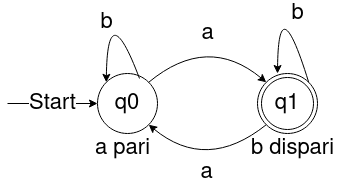
\includegraphics[scale = 0.5]{media/09_21_es1.png}
  \centering
\end{figure}

\item 
stringhe che terminano con bb
\\ SI bb,babb
\\ NO $\epsilon$,ba,a,aba

\begin{figure}[h]
  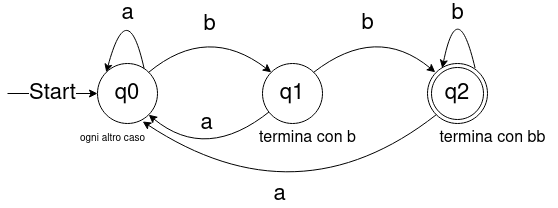
\includegraphics[scale = 0.5]{media/09_21_es2.png}
  \centering
\end{figure}

\newpage
\item stringhe che non terminano con bb
\\ SI $\epsilon$,ba,a,aba
\\ NO bb,babb

\begin{figure}[h]
  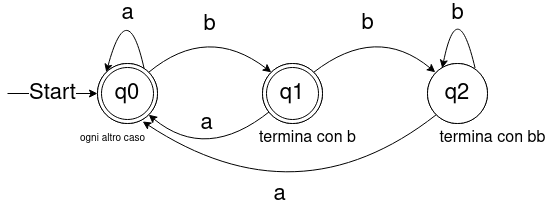
\includegraphics[scale = 0.5]{media/09_21_es3.png}
  \centering
\end{figure}

\newpage
\item stringhe con un numero pari di a ed almeno 3 b
\\ SI bbb,bababb
\\ NO $\epsilon$,bbaa,bababa

\begin{figure}[h]
  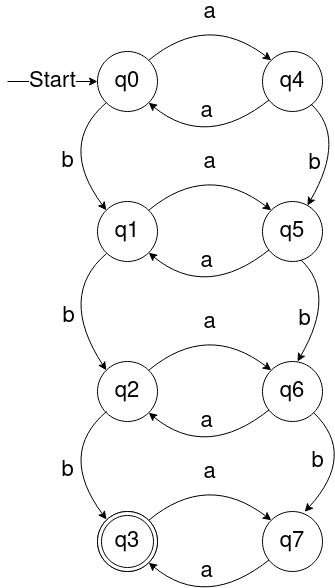
\includegraphics[scale = 0.5]{media/09_21_es4.png}
  \centering
\end{figure}

\newpage
\item stringhe che contengono la sottostringa aaa o la sottostringa aba (contengono almeno una delle due)
\\ SI babab,aaaa,aaaba
\\ NO $\epsilon$,abba,a,b,ab

\begin{figure}[h]
  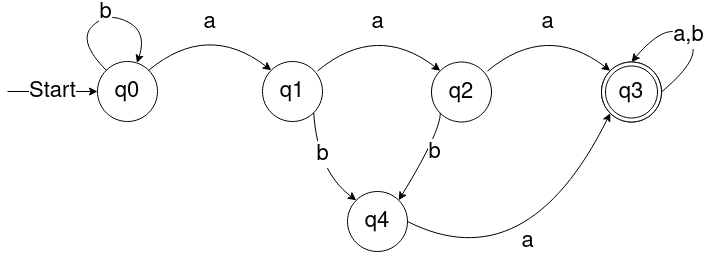
\includegraphics[scale = 0.5]{media/09_21_es5.png}
  \centering
\end{figure}

\item Realizzare un DFA che riconosca il seguente linguaggio su alfabeto \{0,1\}: stringhe che interpretate come numero binario risultano un multiplo di 5 
\\
SI 101,1010,1111,0
\\
NO 111,1,10

\begin{figure}[h]
  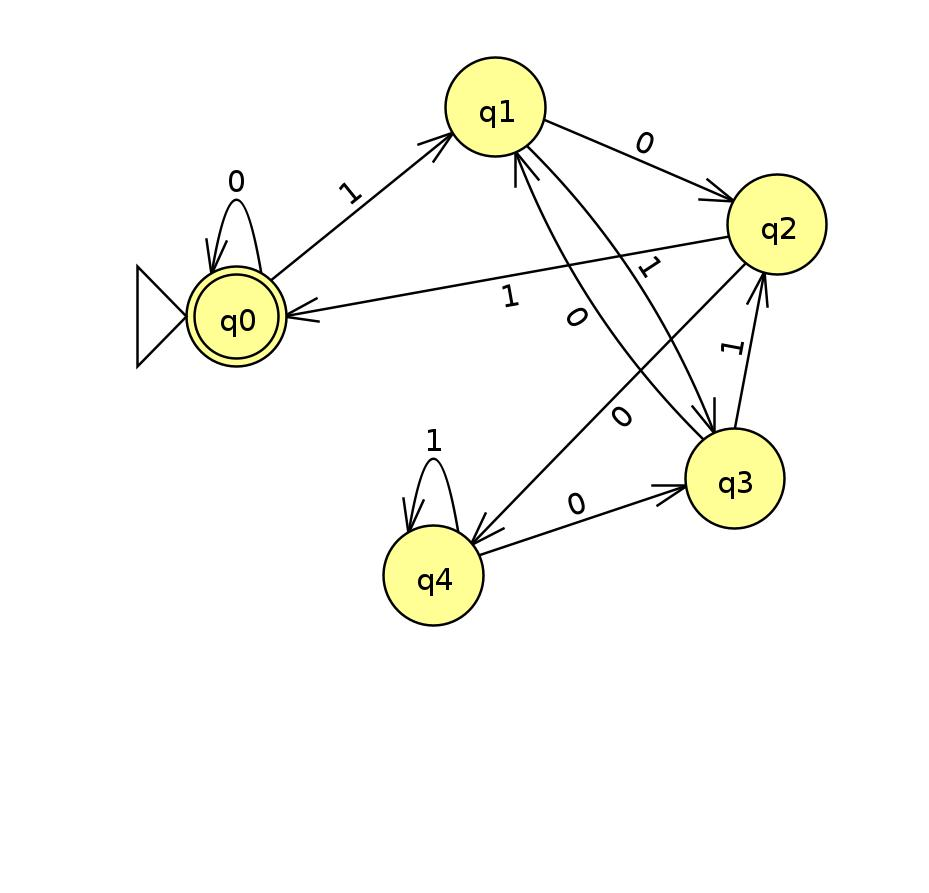
\includegraphics[scale = 0.25]{media/09_21_es6.jpg}
  \centering
\end{figure}
NB: Devi considerare tutti i numeri fino a 5!

\item Sempre considerando alfabeto \{0,1\}, realizzare un DFA che controlla la correttezza delle somme binarie: data la stringa: $a_0 b_0 c_0 a_1 b_1 c_1 ... a_n b_n c_n$ controlla se $a_n...a_1 a_0 + b_n...b_1 b_0 = c_n...c_1 c_0$ (cioè a+b=c con a,b,c numeri binari con stessa lunghezza) 

\begin{figure}[h]
  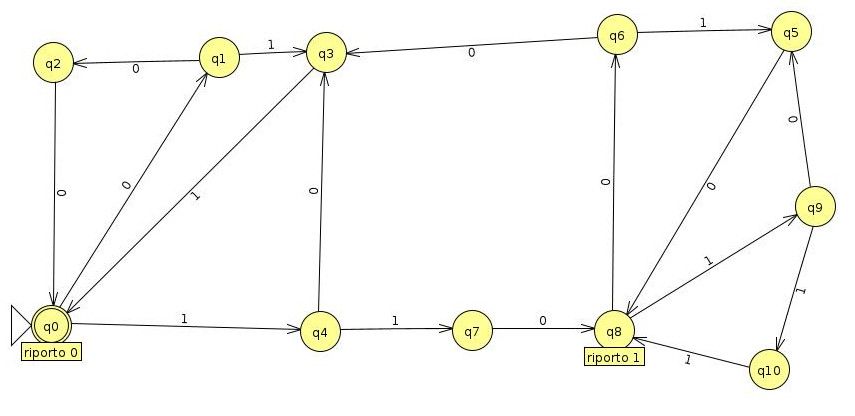
\includegraphics[scale = 0.4]{media/09_21_es7.jpg}
  \centering
\end{figure}

\end{enumerate}

\newpage
\subsubsection{NFA}
\begin{enumerate}
  \item 
    Dato l'alfabeto \{a,b\} realizzare un NFA che riconosce le stringhe che 
    contengono aaa oppure aba
    \\
    SI babab,aaaa,aaaba
    \\
    NO $\epsilon$,abba,a,b,ab

\begin{figure}[h]
  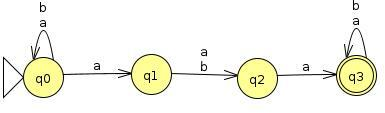
\includegraphics[scale = 0.5]{media/es8.jpg}
  \centering
\end{figure}

  \item Realizzare un NFA che riconosce le stringhe non vuote sull'alfabeto \{0,1,2\} in cui l'ultima cifra appare almeno una volta in precedenza
    \\
    SI 011,121,22,0120
    \\
    NO $\epsilon$,012,20,1

\begin{figure}[h]
  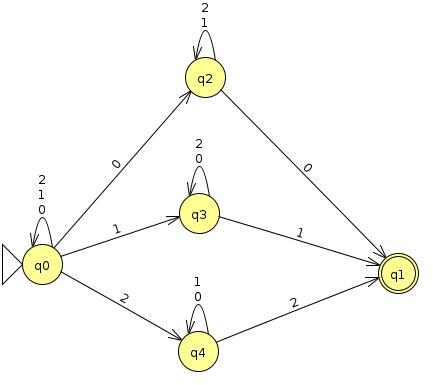
\includegraphics[scale = 0.5]{media/es9.jpg}
  \centering
\end{figure}

\newpage
\item Realizzare un NFA che riconosce le stringhe non vuote sull'alfabeto {0,1,2} in cui l'ultima cifra NON appare in precedenza
\\
SI 012,20,1
\\
NO $\epsilon$,011,121,22,0120

\begin{figure}[h]
  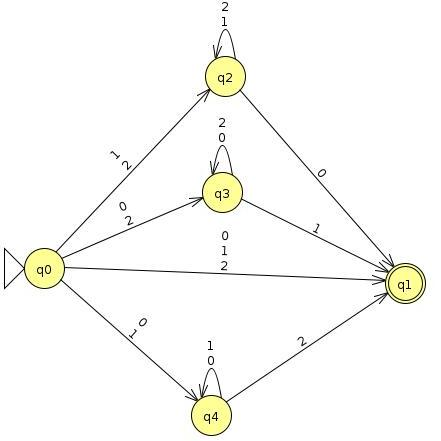
\includegraphics[scale = 0.5]{media/es10.jpg}
  \centering
\end{figure}

\item Dato l'alfabeto {a,b} si consideri l'NFA fatto all'esercizio 1, che riconosce le stringhe che contengono aaa oppure aba. Trasformarlo in DFA.

\begin{figure}[h]
  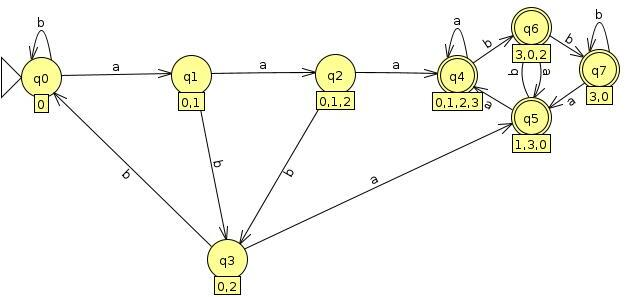
\includegraphics[scale = 0.5]{media/es11.jpg}
  \centering
\end{figure}

\end{enumerate}
